%%%%%%%%%%%%%%%% Conjuntos Imposibles.
\begin{frame}[fragile]{Conjuntos Imposibles:}{Problema.}
  \justifying
  El problema de los \textit{conjuntos imposibles} establece:
  \begin{center}
    \textit{Dado un conjunto con n etiquetas vectoriales de k entradas cada una, decidir si
    es posible o no.}
  \end{center}

  \textbf{Ejemplo:}
  \begin{figure}
    \centering
    \begin{subfigure}[b]{0.3\textwidth}
      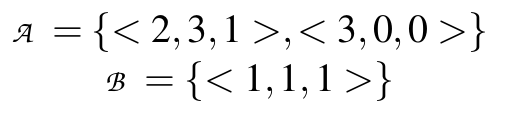
\includegraphics[width=\textwidth]{./Imagenes/Conjuntos}
        \caption{Conjuntos.}
        \label{fig:Conjuntos.}
    \end{subfigure}
    ~ %add desired spacing between images, e. g. ~, \quad, \qquad, \hfill etc. 
      %(or a blank line to force the subfigure onto a new line)
    \begin{subfigure}[b]{0.7\textwidth}
        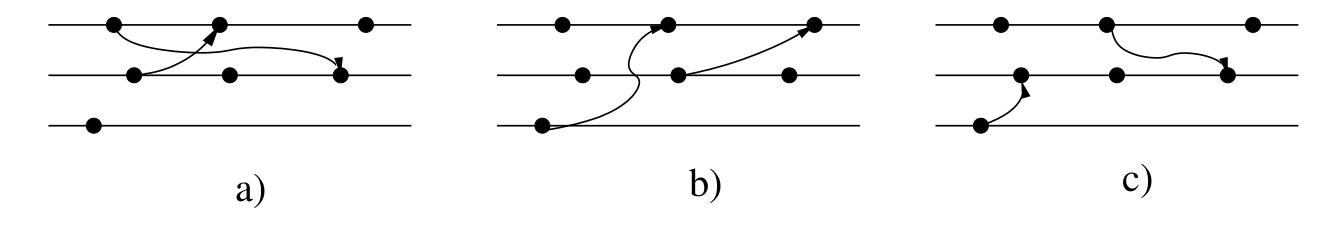
\includegraphics[width=\textwidth]{./Imagenes/Historia}
        \caption{Historias.}
        \label{fig:Historias.}
    \end{subfigure}
    \caption{Detectando conjuntos.}\label{fig:ConjuntosImposibles.}
  \end{figure}
\end{frame}
